\documentclass[notumble,combine]{leaflet}
%\documentclass[a4paper,notumble,combine,debug]{leaflet}
%\usepackage[utf8]{inputenc}
%\usepackage[T1]{fontenc}
%\usepackage{lmodern}
%\renewcommand{\bfdefault}{b}
%\usepackage{microtype}
\usepackage[dvipsnames,usenames]{color}
%\usepackage[dvipdfmx]{graphicx}
%\usepackage[dvipdfmx]{graphicx, color}
\usepackage{graphicx}
\usepackage{alltt}
\usepackage{url}
\usepackage{ascmac}
\usepackage{comment}
\usepackage{here}
\usepackage{wrapfig}
\usepackage{floatflt}
%\usepackage{ifthen}

\makeatletter
% Section color
%% from leaflet.cls
\renewcommand\section{\@startsection{section}{1}{\z@}%
  {-3.5ex \@plus -.75ex}%
  {1ex} %{1.5ex}%
  {\normalfont\Large\sectfont\color{NavyBlue}\addul}}
\newcommand{\addul}[1]{\underline{#1}}
\renewcommand\subsection{\@startsection{subsection}{2}{\z@}%
  {-2.5ex plus -.5ex}%
  {1\p@} %{1ex}%
  {\normalfont\large\sectfont\color{Green}\addul}}
  \renewcommand\subsubsection{\@startsection{subsubsection}{2}{\z@}%
  {-1.5ex plus -.25ex}%
  {0.5\p@} %{1ex}%
  {\normalfont\normalsize\sectfont\color{Emerald}\addul}}
  \makeatother

\graphicspath{{figures/}} 

\title{
	\resizebox{\linewidth}{!}{\bf\color{Orange} スタックチャン}\\
	\vfill
	\parbox[c]{\textwidth}{
\includegraphics[width=\textwidth]{img/stackchan.eps}}\\
%	[\baselineskip]
	\vfill
  \resizebox{\linewidth}{!}{\bf \color{Red} コミュニケーションロボットをあなたの手に。}\\
  \resizebox{\linewidth}{!}{\bf \color{Red} スタックチャンはなにをしなくても、スーパーかわいい}\\
        \vfill
	\resizebox{\linewidth}{!}{\bf スタックチャンコミュニティ}\\
        \resizebox{\linewidth}{!}{{\bf \url{https://scrapbox.io/stack-chan/}}}\\
        \hfill {
\includegraphics[width=2cm]{img/Stackchan_flyer.eps}}\\
}



\date{}
%\CutLine*{1} \CutLine*{2} \CutLine*{3} \CutLine*{4} \CutLine*{5}
%\CutLine*{6}

% \AddToBackground*{2}{% Background of a large page
%   \put(\LenToUnit{.25\paperwidth},\LenToUnit{.4\paperheight}){%
%     \includegraphics[width=14.85cm]{kbug-logo}
% }}


\begin{document}
\maketitle
\thispagestyle{empty}
\pagebreak{}
\section{スタックチャンってなぁに?}
スタックチャンはししかわさんが開発、公開している、 手乗りサイズのスーパーカワイイコミュニケーションロボットです。 
作品ページ:https://github.com/meganetaaan/stack-chan

キャッチフレーズは、以下の通りです。
\begin{itemize}
  \item \resizebox{\linewidth}{!}{\bf\color{Red}コミュニケーションロボットをあなたの手に。}
  \item \resizebox{\linewidth}{!}{\bf\color{Red}スタックチャンはなにをしなくても、スーパーかわいい}
\end{itemize}

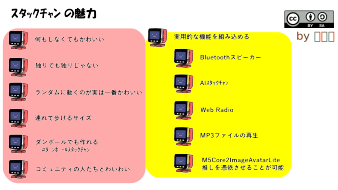
\includegraphics[width=\textwidth]{img/stackchan-salespoint.eps}

\section{スタックチャン3つのオープン}
スタックチャンは、以下の3つのオープンな環境です。
\begin{itemize}
  \item オープンな仕様
  \item オープンなプロセス
  \item オープンなコミュニティ
\end{itemize}

では、各項目を詳しく見ていきましょう。

\subsection{オープンな仕様}
普通の意味でのオープンソースです。

スタックチャンは、ソフトウエアがオープンになっています。
AIやBluetoothスピーカーなどのバージョンのスタックチャンのソースが公開されています。

ハードウエアもオープンになっています。
ハードウエアには、以下のようなものがあります。
\begin{itemize}
  \item 筐体データ(3Dプリント)がオープン
  \item 基板の設計データがオープン
\end{itemize}

\subsection{オープンなプロセス}
スタックチャンは、 制作の過程もオープンになっています。

制作の過程がオープンとは、DiscordやXでスタックチャンの制作例が多数報告されており、自分で製作する時の参考情報が多数手に入ることを意味しています。
ここでは、成功例が手に入るだけでなく、失敗例も手に入るようになっています。

スタックチャンのオープンなプロセスでは、難しいことを難しいと言える雰囲気を大事にしています。


\subsection{オープンなコミュニティ}
 スタックチャンコミュニティは誰にでもひらかれています。

スタックチャンコミュニティでは、全員がユーザーであり開発者でもあります。

うちの子自慢も盛んに行われていますので、あなたのスタックチャン自慢も是非してみてください。

手芸やキーホルダーなどのアクセサリで参加している人たちもいます。

最近は、もくもく会やオンリーイベントなども行われています。
詳しくは、イベント情報をご覧ください。

\section{色々なスタックチャン}
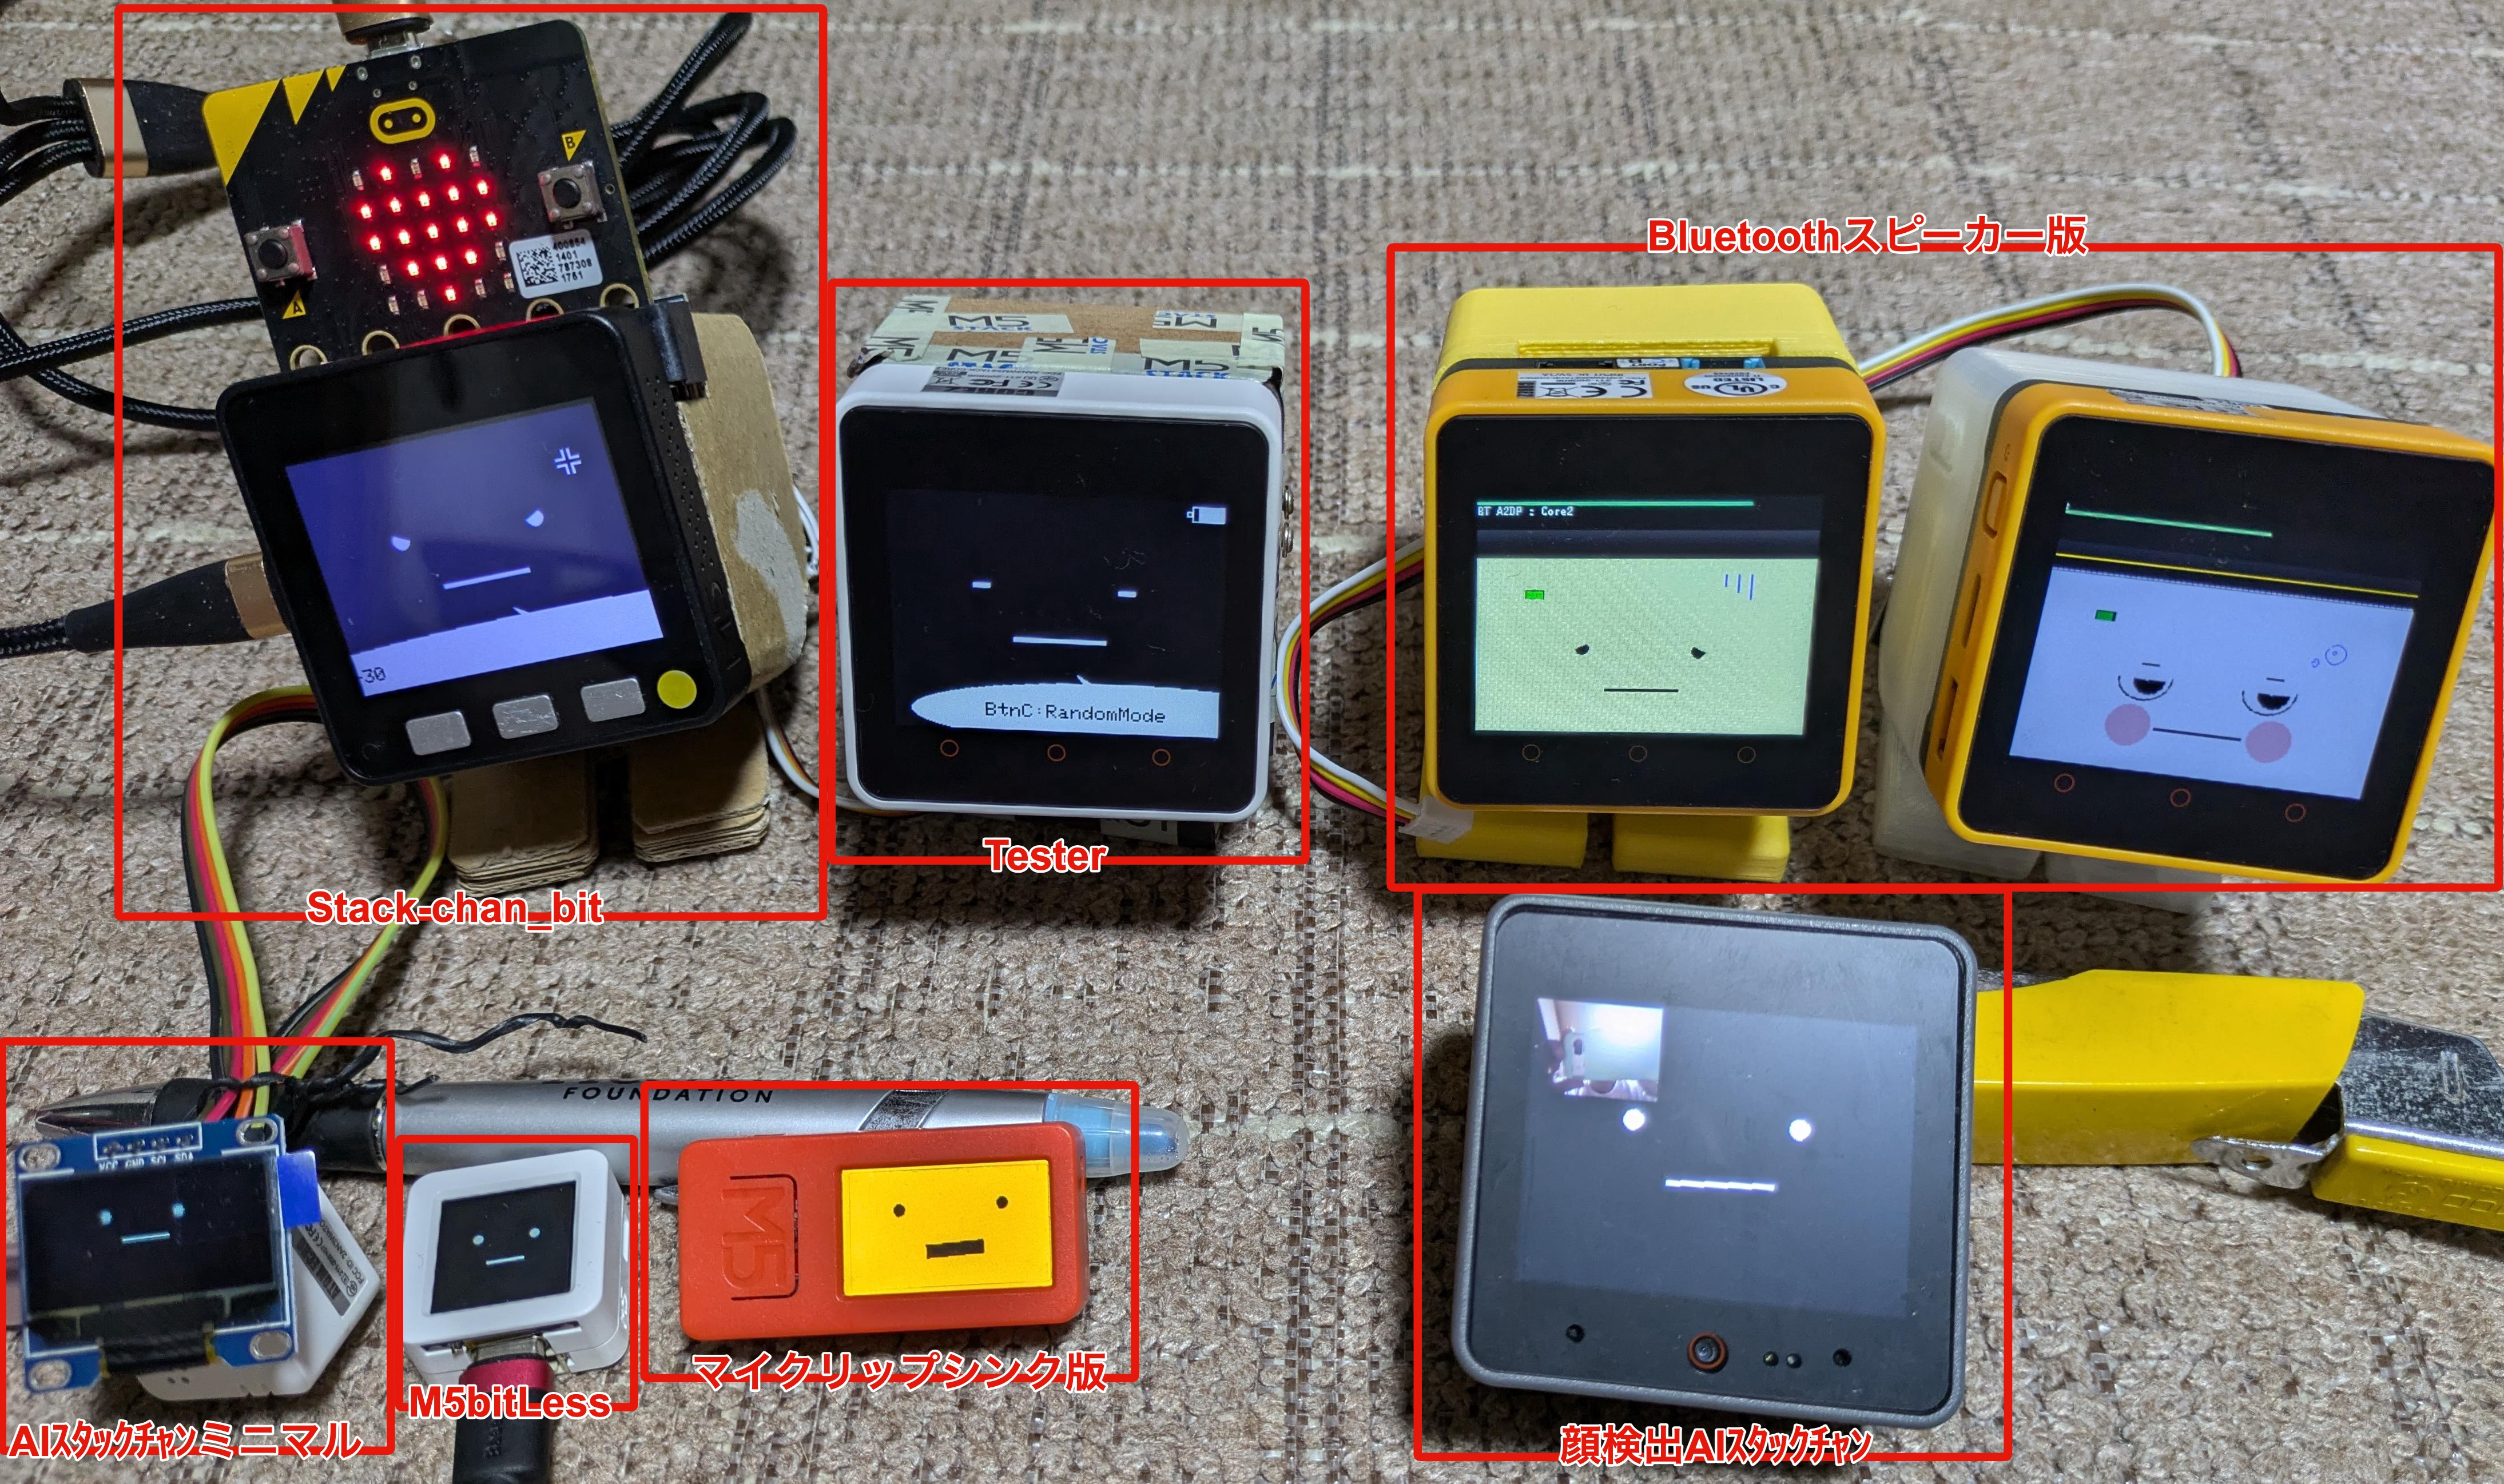
\includegraphics[width=\textwidth]{img/stackchans.eps}
\subsection{Bluetoothスピーカー版}
Bluetoothスピーカー版は、スタックチャンの中でも人気のあるバージョンです。
スタックチャンがBluetoohスピーカーとして動作するため、パソコンやスマートフォンからスピーカーとして利用することができます。
あなたの好きな音楽をかけると、スタックチャンがリップシンクしてまるで歌っているかのように見えます。

\subsection{AI版}
AI版スタックチャンは、スタックチャンがAIとして動作するバージョンです。
スタックチャンが音声で質問を聞いてくれ、ChatGPTなどのAIに問い合わせ、答えを音声で教えてくれます。

\subsubsection{顔検出版CoreS3用AIスタックチャン}
CoreS3という機種では、カメラがついており、顔検出が可能です。
これを使って、顔が検出されるとAI動作がはじまるようになっています。

\subsubsection{AIスタックチャンミニマル}
AIスタックチャンミニマルは、誰にでも気軽にスタックチャンが楽しめるようにというコンセプトで作られたバージョンです。
コストを低く抑えるために、AtomEchoという機種を使い、画面はOLED SSD1306というものを使っています。
現在のところ、5000円程度で作ることができます。

\subsection{Radiko版}
スタックチャンがRadikoプレーヤーになり、ラジオを聞くことができるバージョンです。

\subsection{時計版}
スタックチャンが時計になります。

\subsection{Stack-chan\_bit版}
スタックチャンがmicro:bitから操作できるようになります。
スタックチャン用のMakecode拡張機能が用意されており、簡単にスタックチャンを動かすことができます。

\subsection{動作テスタースタックチャン}
動作テスタースタックチャンは、スタックチャンを作ったときに、まず初めに動作確認をするために使うスタックチャンです。
サーボの調整などに使います。

\section{スタックチャンの作り方}
ここでは、スタックチャンの作り方を簡単にご紹介します。

\subsection{なにを用意したらいいの?}
動くスタックチャンを作るためには、以下のものが必要です。

\begin{itemize}
  \item M5Stack本体
  \item 3Dプリンタで作った筐体
  \item サーボモータと専用基板
\end{itemize}

次に説明するように、M5Stack本体だけでもスタックチャンの基本的な動作をさせることはできますので、まずはここからはじめてはどうでしょうか?

\subsection{お顔だけでも楽しいですよ!!}
スタックチャンの多くのプログラムは、体がなくても動作します。
つまり、M5Stack単体だけで動作するものが多いのです。

たくさんのプログラムが、M5Stack用のプログラム書き込みツールM5Burnerで提供されています。
既に紹介したバージョンのスタックチャンも提供されているので、これを使ってみると良いでしょう。

\subsection{あなたはどのスタックチャン?}
スタックチャンを作成するには、いくつかの選択肢があります。

例えば、M5Stackになにを選ぶのか、筐体をどうするか、サーボモータにどんなものを使うのか、などです。

\newpage
\section{これからの関連イベント(予定)}
\begin{itemize} 
  \item 2025/01/25: OSC 2025 Osakaブース展示 \& LT(オープンソースとスタックチャン)
  \item 2025/02/01: 東京もくもく会@赤坂 オンライン配信あり
  \item 2025/02/15: 神奈川もくもく会@関内 オンライン配信あり
  \item 2025/04/05: スタックチャンオンリーイベント@絶滅メディア博物館(東京)
  \item 未定: 大阪もくもく会@gusuku Ashibinna Osaka(グランフロント大阪)
\end{itemize}

\vfill
\begin{minipage}{\textwidth}
\begin{boxnote}

\section{スタックチャン情報}
スタックチャンに関する情報は、以下のような場所で入手することができます。

\begin{itemize}
  \item Cosense:情報集約用\\
	\url{https://scrapbox.io/stack-chan/}
  \item Dicsord\\
	\url{https://discord.gg/eGhd9adnBm}
  \item X\\
	@stack\_chan(\url{https://x.com/stack_chan})\\
	ハッシュタグ:\#スタックチャン
  \item mixi2:スタックチャンコミュニティ
  \item ProtoPedia:プロトタイプ投稿サイト\\
	\url{https://protopedia.net/material/833}
\end{itemize}


\includegraphics[width=2.2cm]{img/cosense.eps}

\includegraphics[width=2.2cm]{img/discord.eps}

\includegraphics[width=2.2cm]{img/X.eps}

\end{boxnote}
\end{minipage}
2025年1月25日(土)版
\end{document}
